\documentclass[a4paper,11pt,titlepage]{article}
\usepackage{graphicx}
\author{Abrie Greeff\\B.Sc Hons (Computer Science)\\Department of Computer Science\\University of Stellenbosch}
\title{Examination: Cellular Automata with Memory Rules}
\begin{document}
\maketitle
\tableofcontents
\section{Introduction}
This article considers cellular automata with memory rules (CA) as discussed in~\cite{art}. If you are reading this and do not understand any of the concepts please refer to~\cite{art}. I will also assume that you are familiar with all the concepts of the various systems that are discussed. When necessary the basic idea behind every system will be explained.

\section{Implementing Cellular Automata with Memory Rules}
In theory cellular automata with memory rules (historic) may prove to be more efficient for certain CA systems than a normal CA (ahistoric). We will focus on specific implementations in subsequent sections. The first problem that needs to be addressed is how a historic CA will be implemented and that will be the focus of this section.

The CA that we are interested in is a simple two dimensional CA of size n. Each cell in this CA can have two states, zero or one. The reason I am considering this case is because it is the most basic two dimensional CA type and all other types are variations of this basic type.

The ahistoric CA can be represented with a two dimensional 16-bit integer array. The CA would be declared in the following notation,
\begin{verbatim}
int[][] ca = new int[Math.ceil(n/16)][n]
\end{verbatim}
When the CA is declared this way the least space will be used to represent it. To index any given cell \emph{(x,y)} the following call would be made to index the CA,
\begin{verbatim}
cell_value = getBitAt(ca[x/16][y], x%16)
\end{verbatim} The \emph{getBitAt} function is just a hypothetical function that index an integer at position \emph{x mod 16}.

To change this ahistoric CA into a historic CA with memory length of \emph{T} another dimension would be needed to the above array. The following would be the best possible representation,
\begin{verbatim}
int[][][] ca = new int[Math.ceil(n/16)][n][T]
\end{verbatim}
Two extra variables will also be needed to control historic CA. The first will be a counter to count the amount of state changes. Once this amount equals \emph{T} a second boolean variable will be set to let us know we reached \emph{T}. These variables are necessary because until \emph{T} is reached the CA is equivalent to an ahistoric CA. Once \emph{T} has been reached all the cells have enough history to start operating as historic CA. The last problem is how this array would be indexed to obtain the current state and the history. There are two ways of doing this. The first would be to let the first entry be the most current and the remaining entries sorted from newest to oldest. This is the worst method for keeping control of the CA, because for every state change the amount of information that needs to be copied between array entries is very large. To be exact the overhead for every state change would be \emph{$O(Tn^2)$}.

The second option is much more efficient for storing a historic CA. To do this I will use the counter mentioned early as a circular counter. This means every time the counter reaches \emph{T} the counter would be reset to zero. Every time a state change occurs the counter will be incremented and would point to the newest state information. This will mean the oldest information will be replaced every time and no extra copying of data will be needed.

The next thing that is needed is the two bit masks. One for the transition function and one for the history function. I will create the transition mask from a nxn array and the history mask from a T-dimensional array. A set of binary OR and AND operations will then be used to compute the transitions. The other option would be to code specific masks into the program and thus eliminating the extra space. The rest of this section will compare these two methods.

The first method is dynamic, meaning that the masks can be loaded from file. This will allow us to use any possible mask. The advantage of this is that the code needed for the program is very simple. The disadvantages are that the initial loading of the masks is slow and a lot of extra storage space is needed for the extra arrays. If all the main operations on the system are taken in consideration the time complexity for one transition will be $O(n)+O(n)+O(n^2)$.

The second method is static, meaning that the program does only contain one set of masks and can not be altered without the code. The advantages of this is that less space is used and the initial load time is very fast. The disadvantages are that the code is very complex and will take longer to create. Furthermore the system will only support one set of masks. The time complexity for performing all operations for this method will be $O(n^2)+O(1)+O(n^2)$.

Choosing between these methods may prove to be very dependent of the system which it will be programmed for.

\section{DFAs with Memory}
When reading \cite{art} the question is raised whether it is possible to use the idea of memory in deterministic finite automata (DFAs). The first question that we need to ask ourselves is, "Why would we want to use DFAs with memory?". The answer to this question is that we do not know. Then the question needs to be reformulated to, "Why would we not use DFAs with memory?".

To answer this question we need to look at what DFAs are used for. Standard DFAs are a set of states that transition between states based upon information it receives. Here we can see that a DFA does not need memory because once a state is reached we don't need to know what events led to us reaching this state. We only need to know what we want to do when the next information or character is received. If we did use memory when traversing the states and we returned to the first state on a failure the whole system would be traversed again in the same way. Thus adding memory to a standard DFA would not be sensible.

Just because adding memory to a standard DFA is not sensible that still does not mean there is no other types of DFAs that may benefit from having memory. One such type, a DFA with a failure function, will be compared to a DFA with memory. More specifically the Aho-Corasick pattern matching algorithm that uses DFAs with failure functions will be used.

The Aho-Corasick algorithm was developed for reading all patterns in a dictionary. The advantage of the algorithm is that it uses a failure function so that input characters are only read once from the dictionary. I won't go into the detail of how it works, rather see Fig.~\ref{Figure:aho} for an example of an Aho-Corasick DFA. The dotted line represents a failure function.

\begin{figure}[htbp]
   \centering
   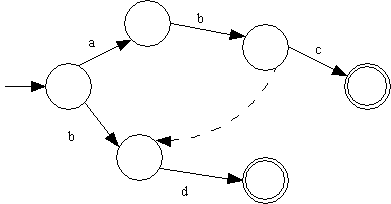
\includegraphics[width=8cm]{aho.png}
   \caption{Aho-Corasick DFA}
   \label{Figure:aho}
\end{figure}

I will try to propose a possible DFA with memory system to improve on Aho-Corasick. Firstly the DFA will be the same as the Aho-Corasick DFA but without the failure function transitions, see Fig.~\ref{Figure:dfa-aho}. The memory of the DFA will be a buffer of characters already read. To make it possible to reach the longest branch the size of the memory should be the amount of transitions in the longest branch of the DFA. When a transition fail the oldest character will be thrown away. The DFA will then be traversed again from the first state to test for the following prefix.
%\newpage
The advantages of this system is that it won't be necessary to construct all the failure functions. The disadvantages would be that unnecessary characters would be read more than once. If one were to compare this to the Aho-Corasick algorithm, one would find that it has the advantages of using less transitions and every character is read only once. It is therefore  practical to choose the Aho-Corasick algorithm over the DFA with memory.

\begin{figure}[htbp]
   \centering
   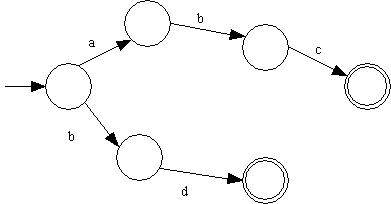
\includegraphics[width=8cm]{dfa.png}
   \caption{DFA without failure function}
   \label{Figure:dfa-aho}
\end{figure}

\section{Improving Robot Path Planning}
Behring's robot path planning algorithm works in three phases. The first phase is the initial configuration phase. In this phase the terrain for the area the robot has to traverse is loaded. It also includes the robot's initial position and its goal position.

In the second phase the area is flooded and the Manhattan distance is calculated of each cell. This flooding is done from the goal position until the initial position is reached. The third phase is when the robot traverses the area by following the shortest distance to the goal position.

We want to know that by changing the ahistoric CA, used to implement the algorithm, to a historic CA if the system would be more efficient. If the system is changed to accommodate a historic CA then it needs to be checked if any of the three phases show improvement and if any show worse performance.

In the first phase it would not be necessary to add memory because this phase consists of only one state change, the state change between an empty configuration and the initial configuration. If the historic CA was used it would only decrease the performance because of the extra space needed to store a historic CA.

The second phase has one state change at the most for every cell in the CA. This happens when a cell's Manhattan distance is set to a value. The historic CA would therefore once again only waste valuable system memory. The last phase has no state changes and therefore a historic CA would once again only be a waste of memory.

The historic CA does not improve the performance of Behring's robot path planning algorithm in any way and only increases the space complexity. The reason for this is the small number of state changes that occur in this system. If one would want to improve the algorithm the best way is to find a method that would improve the time needed to flood the whole CA.

\section{Improving Random Number Generators}
Tausworthe random number generators are generated from a binary n-dimensional CA. To add memory to these CAs is easy and the same as the systems shown in \cite{art}. By adding memory to the Taustworthe generator is the same as the normal generator but the last \emph{T} values are now remembered. We have seen in \cite{art} that historic CA's cells are more active than there ahistoric counterparts. For this specific application of historic CAs we are hoping to obtain longer cycles.

Cycles are the amount of numbers that are generated before the numbers start repeating again. The better the rules are for a Tausworthe generator, the bigger the cycles get. Thus we want to know if adding memory to Tausworthe generators will improve the cycle length. In theory this is not possible. The reason I am saying this is because if adding memory would improve the length of a cycle then it is always possible to define a rule that would have the same cycle length. 

There exists a rule that would have the longest possible cycle but no one has been able find this rule. If we look at this in theoretical manner and say that someone found the rule with the longest possible cycle and also a Tausworthe generator with memory that generated the same cycle. This is the only possible way to compare these two methods.

The historic CA would have no advantages over the ahistoric CA. It will however have disadvantages. The historic CA would need more space in memory and it would much slower. We can see this if we compare the time complexity between the two. The historic CA would run in \emph{$O(Tn)$}, while the ahistoric CA would run in \emph{$O(n)$}. The space complexity of the two also tell the same story. The historic CA needs \emph{$O(Tn)$} and ahistoric CA needs \emph{$O(n)$}. Even if a historic CA may improve a current implementation, the disadvantages are enough to stay with the current implementation.

\section{Extending to a Non-Linear Case}
All the systems that were discussed so far uses linear rules. This means they are rules that can be represented by linear functions. In this section I will be considering if historic CA can be developed for systems that have non-linear rules. More specifically I will be considering if it will be possible to extend a data-encryption system using exclusive-not-or nondeterministic finite automata (XNOR-NFAs).

Implementing non-linear rules for a historic CA should not be a problem. However we have seen in the previous sections that even if a historic CA system can be developed that still does not mean it will work or be sensible for a specific CA system. Rather than try to explain why it will be possible to develop a historic CA for non-linear rules, I will try to extend the XNOR-NFA system to include a memory property.

Before it is possible to extend the XNOR-NFA system we need to find what in the system can be extended to include a memory attribute. The first thing we need when constructing the encryption system is a NFA. This NFA will be transformed into a equivalent DFA using subset construction and applying the binary XNOR operation on the original NFA. Fig.~\ref{Figure:nfa} is the original NFA's transition table and the equivalent DFA's transition table. This DFA's transition table is then used to obtain circular cycles which are used in encryption and decryption.

\begin{figure}[htbp]
   \centering
   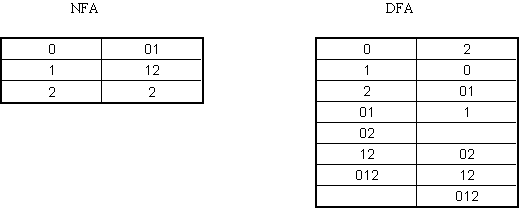
\includegraphics[width=8cm]{nfa.png}
   \caption{NFA and DFA transition tables}
   \label{Figure:nfa}
\end{figure}

The problem is now extending this system to include memory attributes. When viewing through the steps taken in the construction it becomes evident that the only place a memory attribute can be added would be when the DFA is constructed from the NFA. This is also the step where the non-linear rules are applied. This step will be the obvious choice in adding the memory attribute. However it remains to be seen if adding a memory attribute will affect the circular cycles created by the original implementation.

I chose the memory attribute to add the transitions of the entries on the other side of the transition table. For example if we take the first entry in the NFA transition table of \ref{Figure:nfa} the memory attribute would add the transition functions of 0 and 1 to 01 before the XNOR operation would be performed. The subsequent DFA that is then constructed will be as in Fig.~\ref{Figure:newnfa}.

\begin{figure}[htbp]
   \centering
   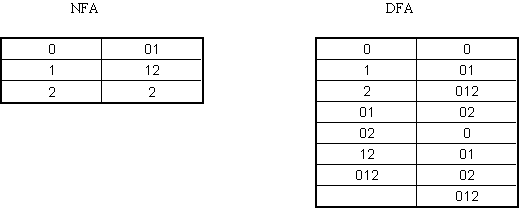
\includegraphics[width=8cm]{new.png}
   \caption{NFA and DFA transition tables with memory}
   \label{Figure:newnfa}
\end{figure}

If this implementation will work the cycles will need to be even. Fig.~\ref{Figure:cycle} shows the original cycles and the new cycles with the memory attribute. As can be seen from this example the encryption system using the memory attribute will not work because it is impossible to decrypt data from the cycles that is formed from this DFA. Therefore extending the XNOR-NFA system by adding a memory attribute is not a viable option.

\begin{figure}[htbp]
   \centering
   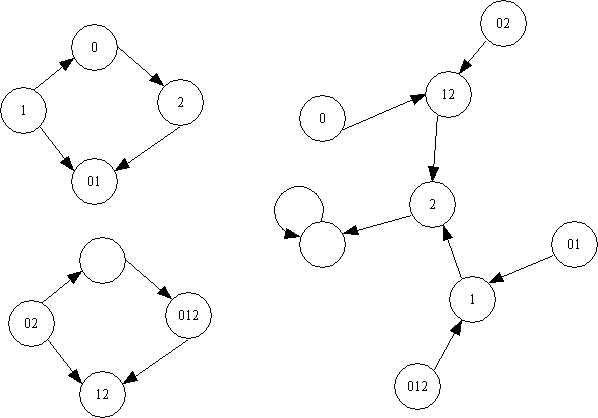
\includegraphics[width=8cm]{cycle.png}
   \caption{Cycles}
   \label{Figure:cycle}
\end{figure}
\newpage
\section{Statecharts with Memory Rules}
Statecharts are an extension to DFAs that allow occlusion by allowing different levels of detail to be separated from each other. My implementation uses threads to create the DFAs that represent each level.

The last topic we will be discussing is whether it is viable to add another extension to DFAs by adding memory rules. We have already seen in Section 3 that a normal DFA does not need memory rules because the history of what happened is not necessary. We now ask why would a statechart need to know what happened before it reached a certain state in the system.

If one looks at the problem it seems evident that memory rules is not necessary because every level is just a normal DFA. There is however instances where it may be necessary to know what happened so far. Statecharts are used to model real-time systems. What if a life critical that should not fail under any circumstances fail. If memory is added to such a system when it is being tested it may store a history of the last \emph{T} events that occurred before the system failed. This may enable the designer of the system to locate a life threatening problem in his system.

This is the only evident reason that memory rules may be used in conjunction with statecharts. This is a good example of where the designer of a system needs to decide beforehand if the failure of his system is important to him.

\begin{thebibliography}{9}
\bibitem{art} R Alonso-Sanz, M Martin,
\emph{Elementary Cellular Automata with Elementary Memory Rules in Cells: The Case of Linear Rules}, Journal of Cellular Automata, Vol. 1, pp. 71-87.
\end{thebibliography}
\end{document}
